\documentclass[11pt,a4paper,twoside]{book}

\usepackage{cover}
%======================================================================
% Use package
\usepackage{graphicx}
\usepackage {subfigure}
\usepackage {hhline}
\usepackage{color}
\usepackage{amsmath}
\usepackage{amsfonts}
\usepackage{amssymb}
%\usepackage{ulem}
%\usepackage{fancyheadings}
\usepackage{fancyhdr}
\usepackage{placeins}
\usepackage{array}
\usepackage{tabularx}
\usepackage{cite}

%======================================================================
% EN-TETES ET PIEDS DE PAGE
\pagestyle{fancy}
\addtolength{\headwidth}{\marginparsep}
\addtolength{\headwidth}{\marginparwidth}
\renewcommand{\chaptermark}[1]{\markboth{\thechapter\ #1}{}}
\renewcommand{\sectionmark}[1]{\markright{\thesection\ #1}}
\fancyhf{}
\fancyhead[LE,RO]{\thepage}
\fancyhead[LO]{\rightmark}
\fancyhead[RE]{\leftmark}

\fancypagestyle{toto}{
\fancyhead{}
\fancyhead[LE,RO]{\thepage}
}

%======================================================================
% CHANGE LES POLICES POUR LES TITRES DES SECTIONS
\usepackage{sectsty}
\allsectionsfont{\sffamily}

%======================================================================
% STYLES DES PARAGRAPHES
\parindent 0em % Permet de commencer les paragraphes au d�but de la marge
\parskip 1.8ex plus 0.0ex minus 0.5 ex
\renewcommand{\baselinestretch}{1.1}


\begin{document}
%============
% Permet d'avoir une autre num�rotation pour le d�but du document
\frontmatter

%============
% Display the cover and table of content

% \version{0.11RC}
% \datenow{31. April 2004}
\version{0.18}
\datenow{18. February 2007}
\makecover
\newpage\thispagestyle{empty}\addtocounter{page}{-1}
~\newpage\thispagestyle{empty}\addtocounter{page}{-1}
%\makecover
%\newpage\thispagestyle{empty}\addtocounter{page}{-1}
%~\newpage\thispagestyle{empty}\addtocounter{page}{-1}
\tableofcontents

%=========
% Start the correct numbering now
\mainmatter

\chapter{Overview}

RAT is developed in IDL\cite{web:idlvm}.

Official publications about RAT \cite{reigber04:rat, neumann05:rat, neumann07:rat}.


\include{type_of_data}
\chapter{The FILE menu}
%=============================================================
\begin{figure}[!htbp]
   \centering
   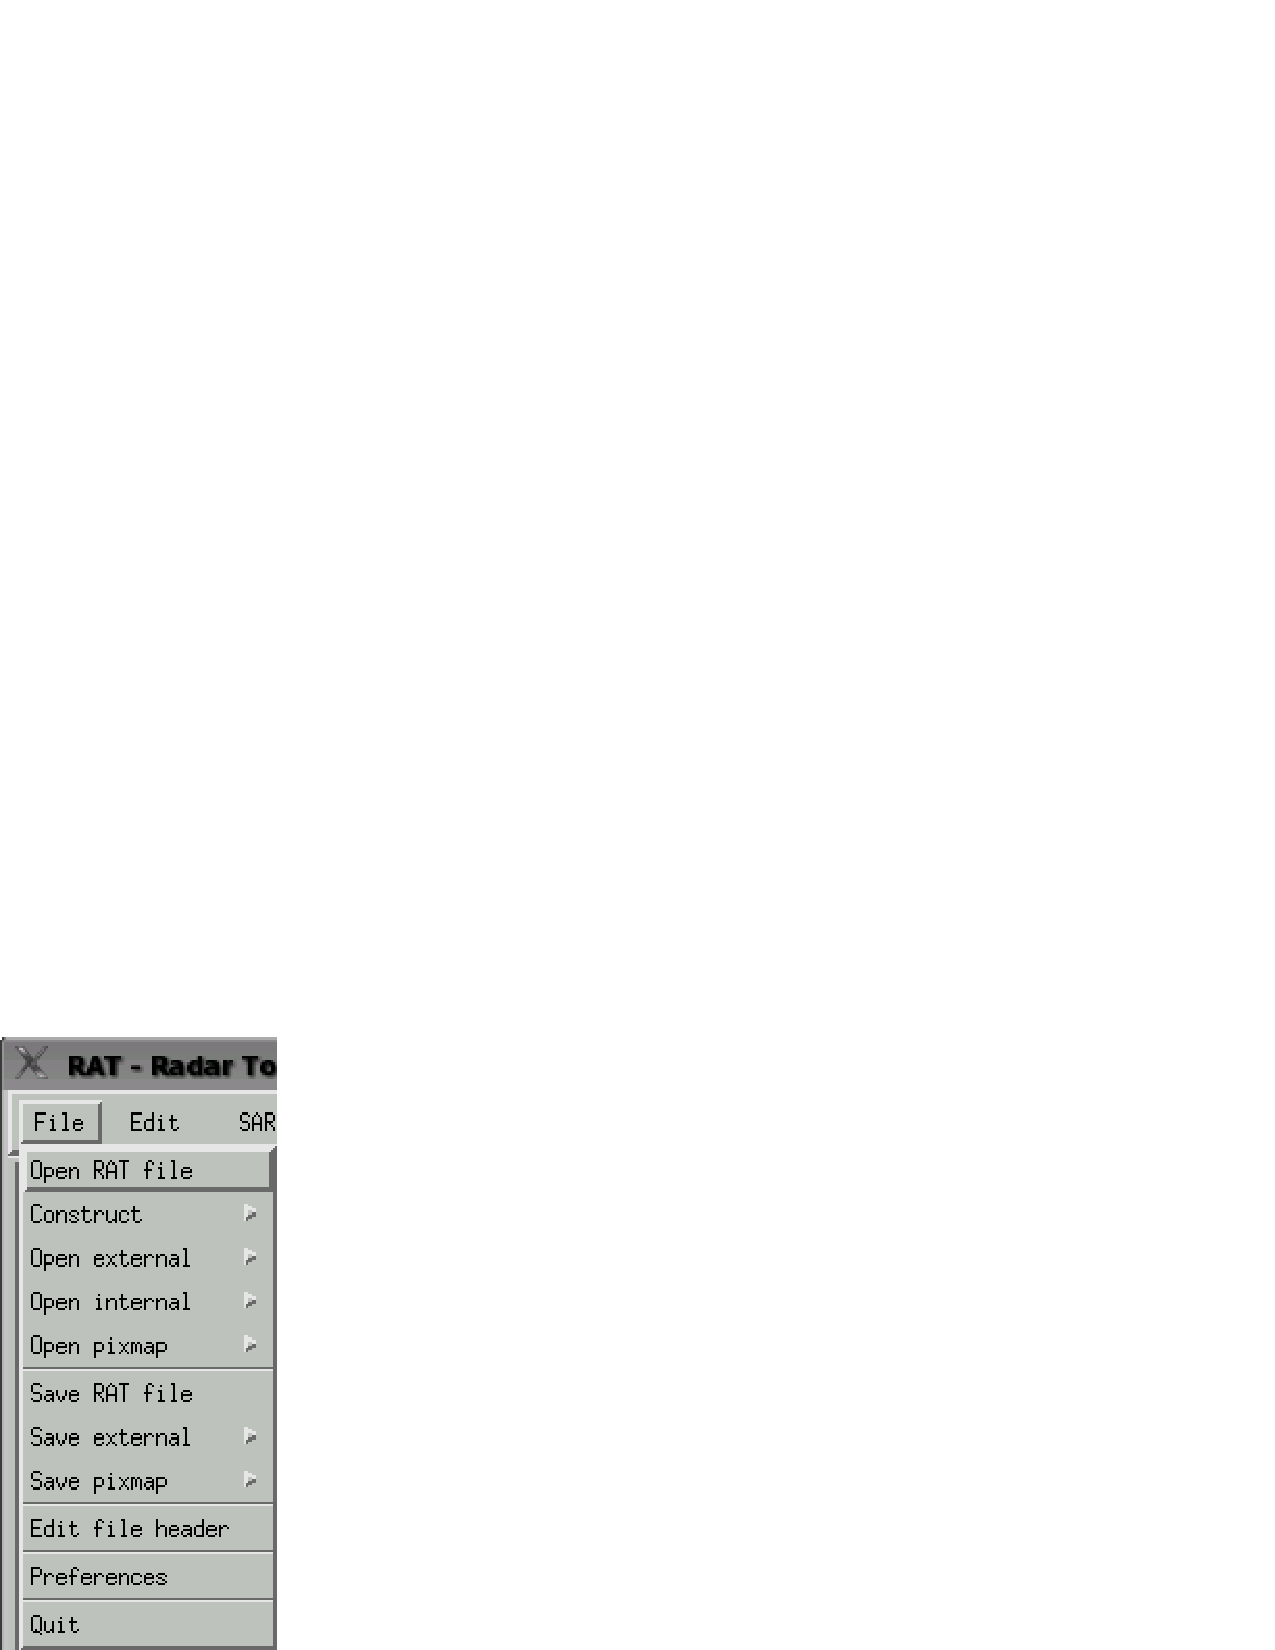
\includegraphics[scale=0.8]{images/pdf/file_menu.pdf}
\end{figure}

Use the \textbf{\textit{File}}  menu on the RAT menu bar to read files into RAT, save file, construct polarimetric or interferometric images, import or export into different data formats, set preferences, edit the file header of the RAT file format and exit RAT.

%=============================================================
\newpage 
%=============================================================
%=============================================================
\section{Open RAT file}
Use the ``Open RAT file'' to open data saved in RAT format.

\subsection{RAT file format}

RAT uses a special file format, containing information about data type, size and representation. Until some import filters are available, you'll have to convert your data to RAT format before beeing able to work with it. This is quite simple if you know how to use IDL. If not, have a look at the format description. In fact, the RAT format is just a simple header plus the data in binary representation.

\subsection{How to generate a file in RAT format with IDL}

Quite easy:
 
\begin{itemize}
	\item Enter IDL
	\item Compile RAT or restore the IDL save-file. This makes a routine for writing RAT files available (srat).
	\item Read your data into an IDL variable using your own rotines. You should know how....
	\item Write the RAT file with the command \verb*|srat,"file.rat",var| on the IDL command line. 'file.rat' denotes the RAT file to be generated, `var' the variable in which contains your data.
	\item Now you can start RAT and load the content of the file  with File$>$Open RAT file.
\end{itemize} 

\subsection{RAT format description}

A RAT-file is structured as in the following:

\begin{center}
\begin{tabular}{|c|c|p{10cm}|}
\hline 
Element & \textbf{type} & \textbf{Description} \\ 
\hline
\hline
DIM & 1*long integer & Number of dimensions of the array \\
\hline
SIZE & DIM*long integer & Array sizes for each dimension \\
\hline
VAR & 1*long integer & Type of Array (1=byte, 2=int, 3=long, 4=float, 5=double, 6=complex, 9=double complex) \\
\hline
TYPE & 1*long integer & Type of Data (100 = SAR amplitude image, 101 = SAR complex image, etc.... (see definitions.pro) \\
\hline
DUMMY & 3*long integer & Reserved \\
\hline
INFO & 80*byte & Comment string \\
\hline
ARRAY & Array type & The array itself \\
\hline 
\end{tabular}\\
\end{center}

%=============================================================
\newpage 
%=============================================================
%=============================================================
\section{Construct}
\subsection{InSAR pair}
\subsection{PolSAR pair}

%=============================================================
\newpage 
%=============================================================
%=============================================================
\section{Open external}
\subsection{E-SAR (DLR)}
\subsection{ENVISAT-ASAR}
\subsection{Radarsat-2}
This routine is made for importing RADARSAT-2 data in Geo-TIFF format into RAT.
Up to now, it has been only tested using simulated data - RADARSAT-2 is not yet
in space!

Basically, this routine has only two options: Reading quad-pol data, i.e. data
composed out of the four polarisation HH,VV,HV and VH, or single-pol data. Since
RAT does not support partial polarimetry, dual-pol data are threated as two
individual single-pol files. When reading quad-pol data, only one of the four files
has to be selected in the fileselector. RAT will automatically find the 3 others.
When not all the 4 files are found, RAT switches back to single-pol.

Many thanks to Daniel De Lisle from CSA for providing a CD with simulated sample
data.

\subsection{PolSARPro}
\subsection{Generic binary}
\subsection{ENVI standard}

%=============================================================
\newpage 
%=============================================================
%=============================================================
\section{Open internal}
\subsection{rarr / sarr}
\subsection{2*long + complex}
\subsection{E-SAR-RK (Rolf)}

%=============================================================
\newpage 
%=============================================================
%=============================================================
\section{Open pixmap}
\subsection{Open PNG}
\subsection{Open JPEG}
\subsection{Open TIFF}

%=============================================================
\newpage 
%=============================================================
%=============================================================
\section{Save RAT file}

%=============================================================
\newpage 
%=============================================================
%=============================================================
\section{Save external}
\subsection{ENVI Standard}
\subsection{Generic binary}

%=============================================================
\newpage 
%=============================================================
%=============================================================
\section{Save pixmap}
\subsection{Save PNG}
\subsection{Save JPEG}
\subsection{Save TIFF}

%=============================================================
\newpage 
%=============================================================
%=============================================================
\section{Edit file header}

%=============================================================
\newpage 
%=============================================================
%=============================================================
\section{Preferences}

%=============================================================
\newpage 
%=============================================================
%=============================================================
\section{Quit}

%  
%  %=============================================================
%  \newpage 
%  %=============================================================
%  %=============================================================
%  %=============================================================
%  \section*{Construct}
%  \addcontentsline{toc}{section}{Construct}
%  
%  \begin{center}
%  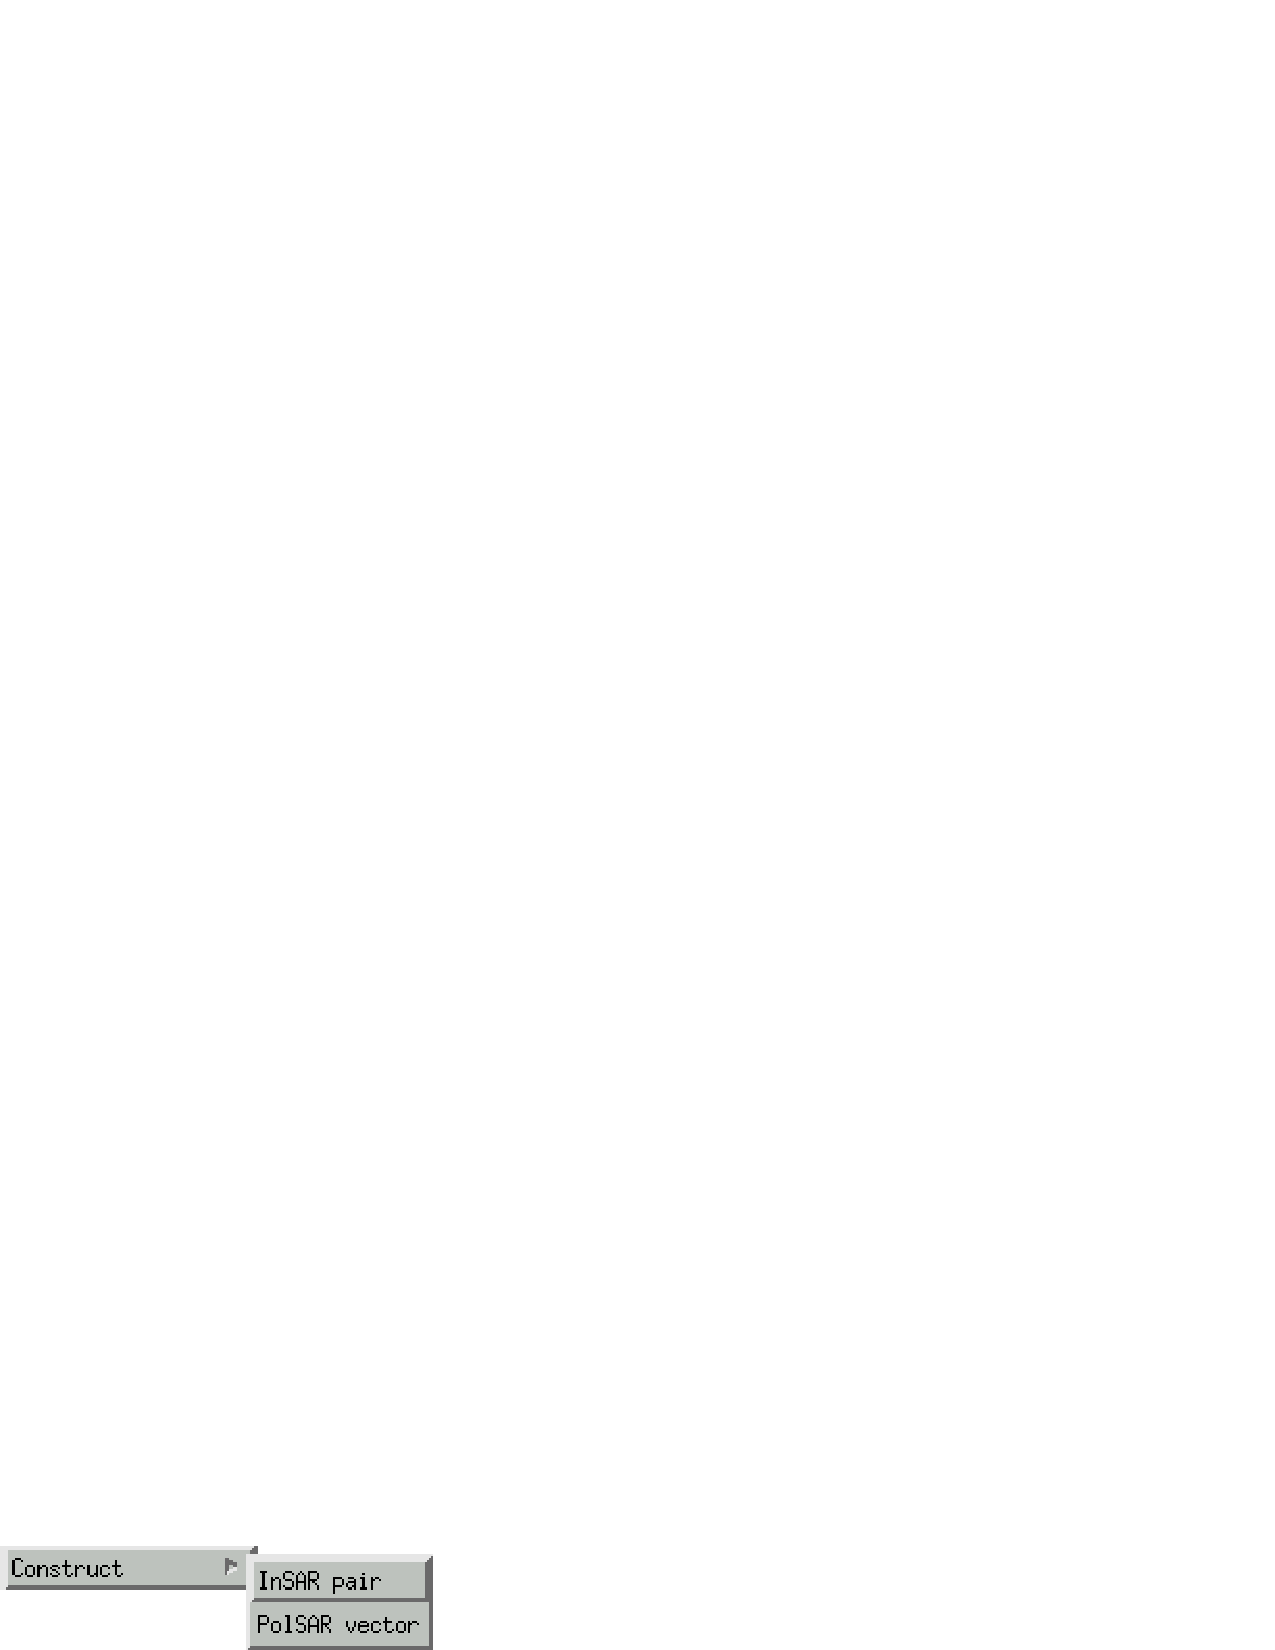
\includegraphics[scale=1]{images/pdf/construct.pdf}
%  \end{center}
%  
%  There are two options for this menu:
%  
%  \begin{itemize}
%  \item Construct InSAR pair, to generate an interferometric data vector
%  
%  \item Construct PolSAR vector, to generate an polarimetric data vector
%  \end{itemize}
%  
%  %=============================================================
%  \newpage 
%  %=============================================================
%  %=============================================================
%  %=============================================================
%  \section*{Construct InSAR pair}
%  \addcontentsline{toc}{section}{Construct InSAR pair}
%  
%  \begin{center}
%  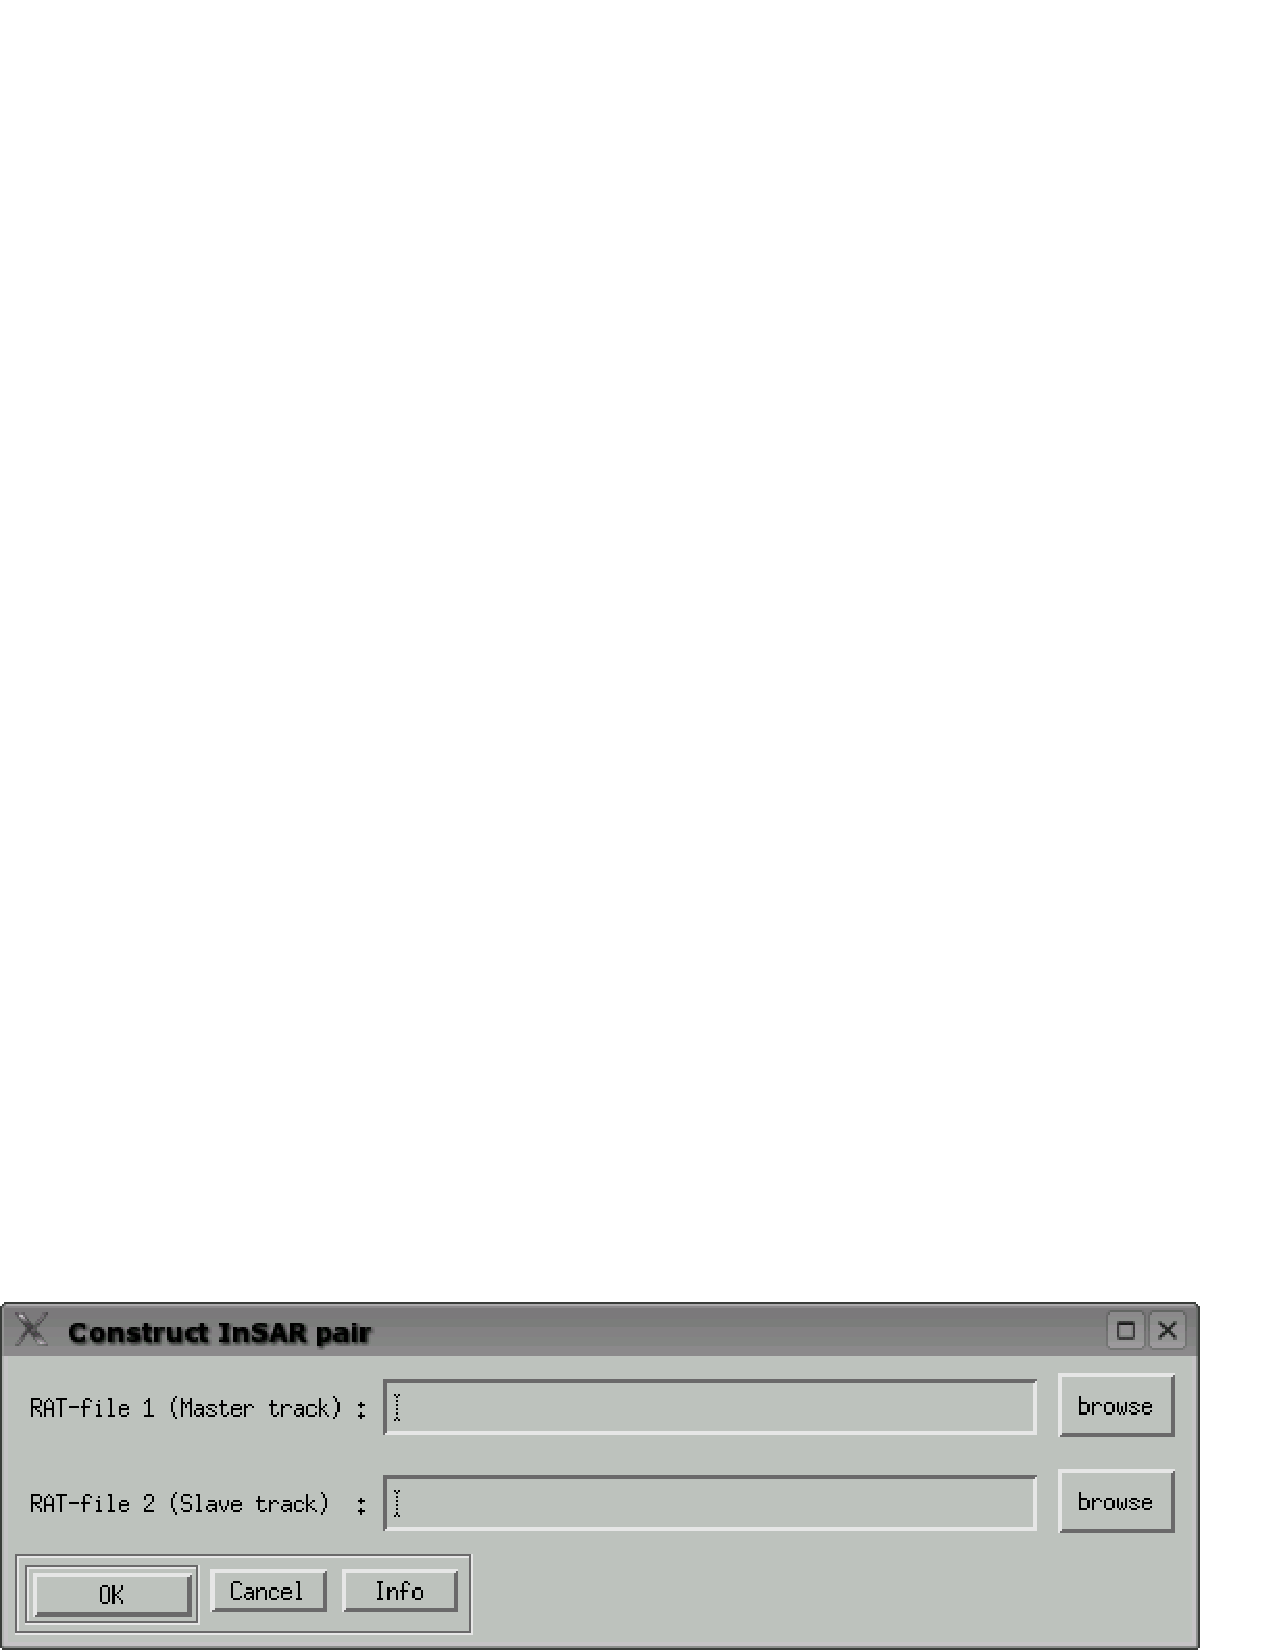
\includegraphics[scale=0.8]{images/pdf/construct_insar.pdf}
%  \end{center}
%  
%  To construct an InSAR pair data, you need two SAR images. The input files have to be in the RAT format, otherwise you will get an error message.
%  
%  The first file correponds to the reference interferometric track, also called ``master track'' and the second file corresponds to the dependant file, also called ``slave track''. 
%  
%  %=============================================================
%  \newpage 
%  %=============================================================
%  %=============================================================
%  %=============================================================
%  \section*{Construct PolSAR vector}
%  \addcontentsline{toc}{section}{Construct PolSAR vector}
%  
%  \begin{center}
%  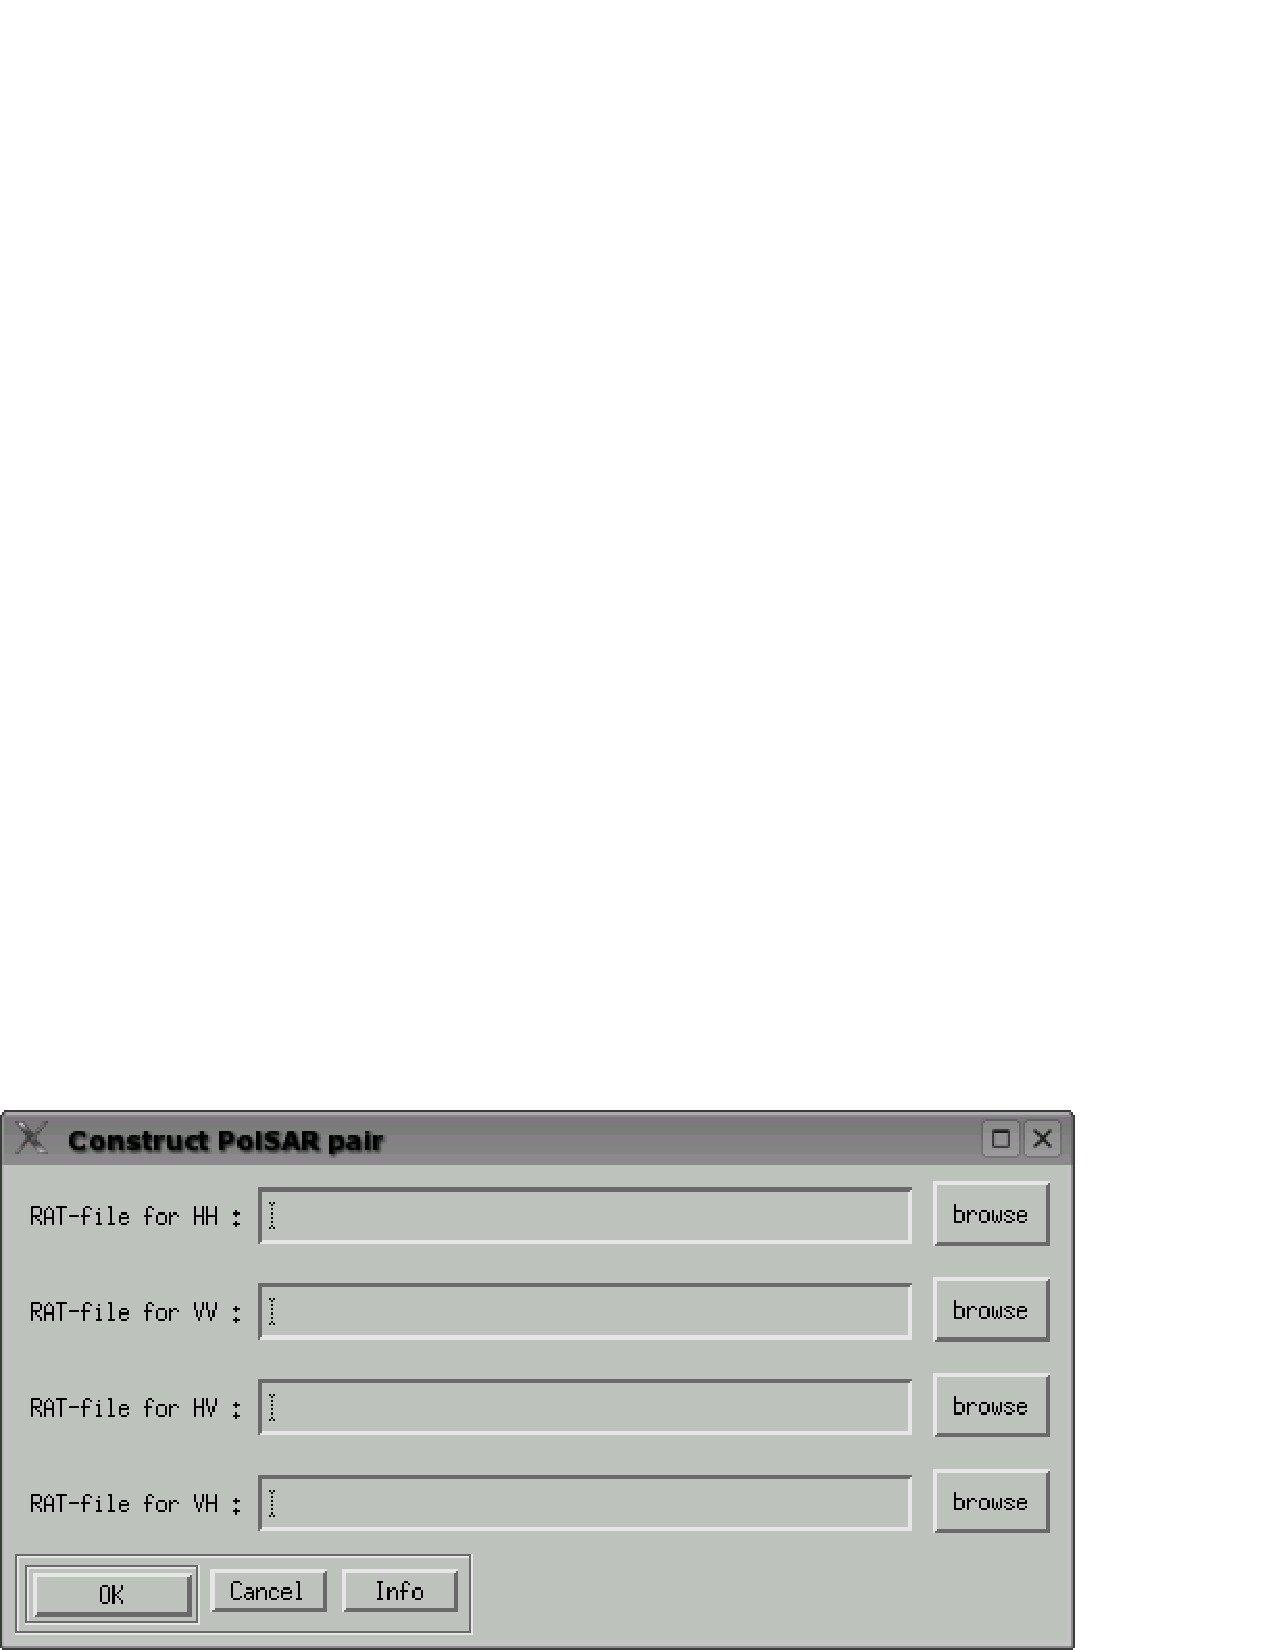
\includegraphics[scale=0.8]{images/pdf/construct_polsar.pdf}
%  \end{center}
%  
%  To construct a PolSAR vector you need, at least, 2 SAR images. The input files have to be in the RAT format, otherwise you will get an error message.
%  
%  The two first RAT--file are obligatory. By construction of RAT, the polarisation channel used should be in the horizontal/vertical basis. The first file is in polarisation HH and the second file is in polarisation VV.
%  
%  The two last files are optional. First you can add a HV channel, then, a VH channel.
%  
%  %=============================================================
%  \newpage 
%  %=============================================================
%  %=============================================================
%  %=============================================================
%  \section*{Open external}
%  \addcontentsline{toc}{section}{Open external}
%  
%  \begin{center}
%  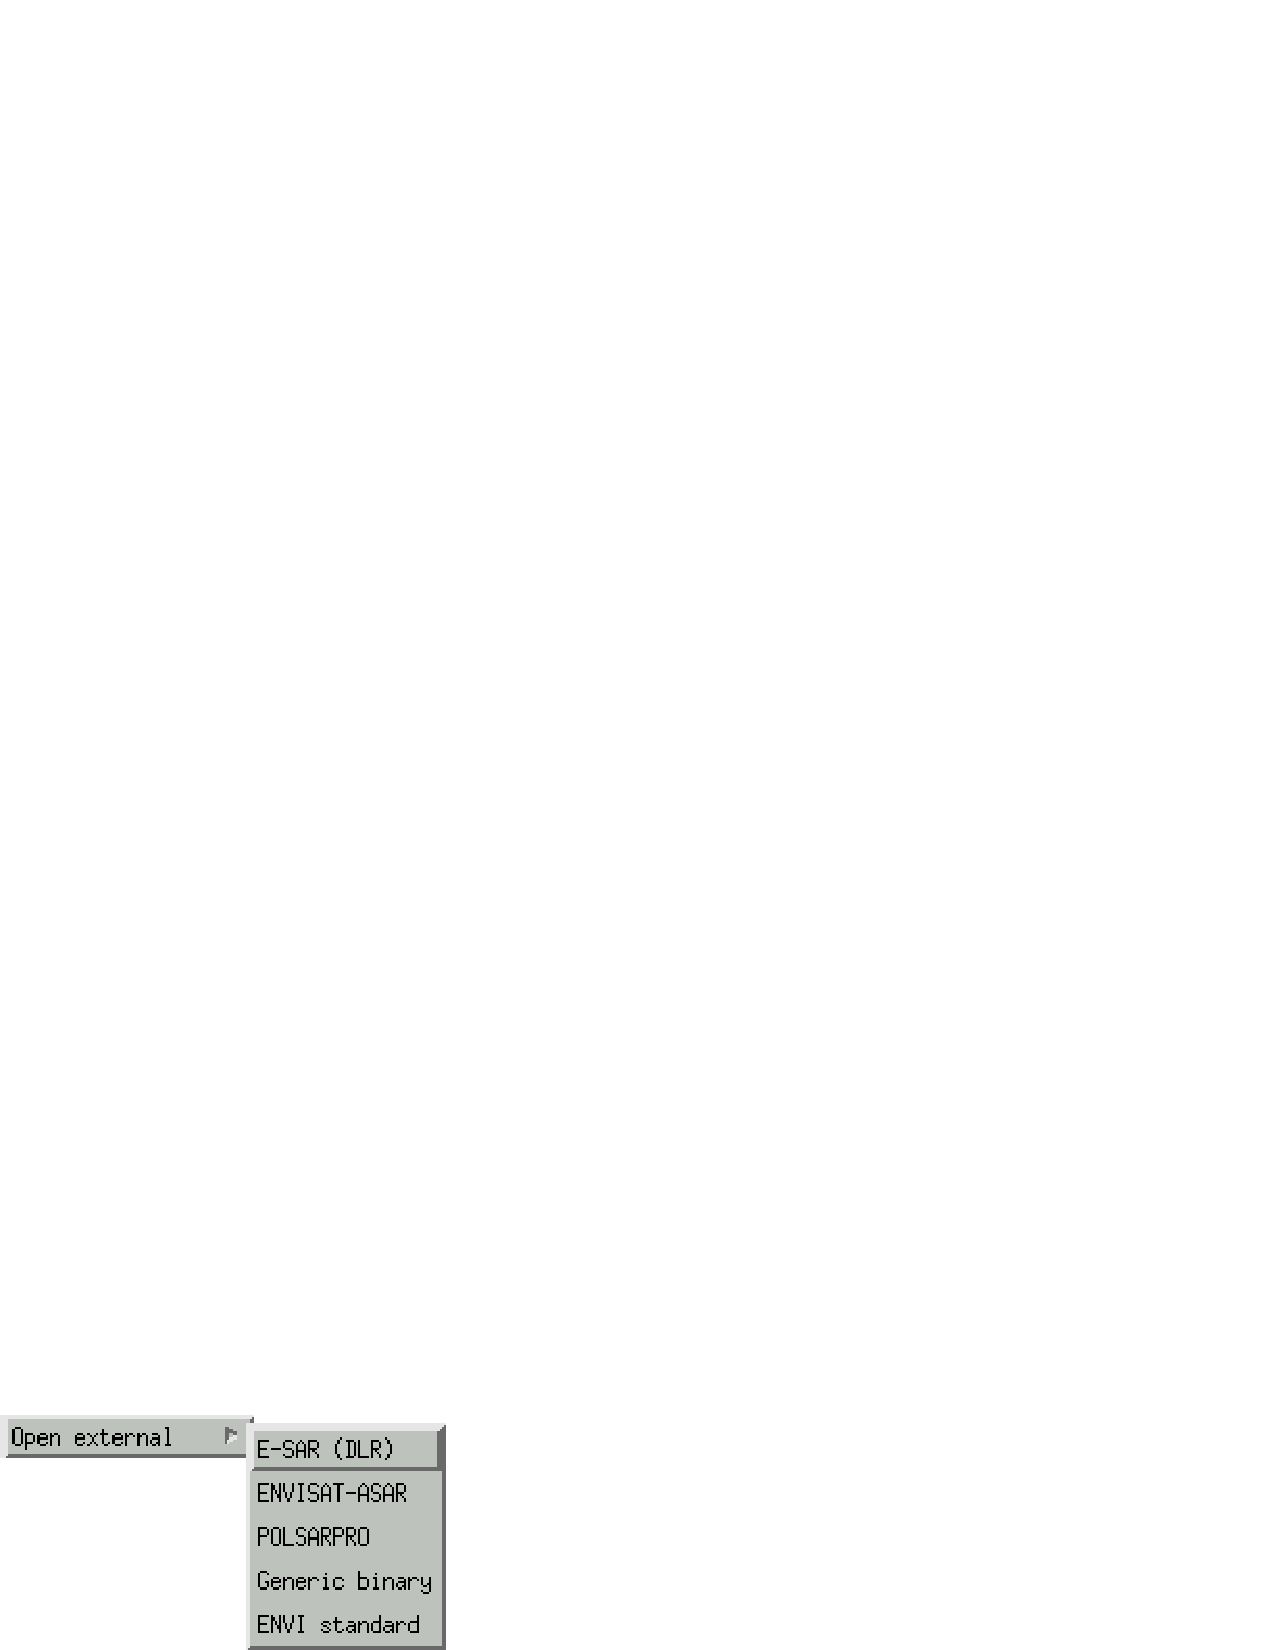
\includegraphics[scale=1]{images/pdf/open_external.pdf}
%  \end{center}
%  
%  There are five options for this menu:
%  
%  \begin{itemize}
%  \item E--SAR (DLR): open file data provided by the E--SAR sensor from the DLR.
%  
%  \item ENVISAT--ASAR: open file data provided by ENVISAT--ASAR.
%  
%  \item POLSARPRO: open file data provided by the software POLSARPRO
%  
%  \item Generic binary: open generic data file. You can specify lot of parameters
%  
%  \item ENVI standart: open envi standart file (only envi standart file)
%  \end{itemize}
%  
%  %=============================================================
%  \newpage 
%  %=============================================================
%  %=============================================================
%  %=============================================================
%  \section*{Open ESAR}
%  \addcontentsline{toc}{section}{Open ESAR}
%  
%  This option allows you to open a SAR data processed by the DLR. This function is based on filename analysis.
%  
%  If the format is recognise, the procedure function ask you for different more informations.
%  
%  %=============================================================
%  \newpage 
%  %=============================================================
%  %=============================================================
%  %=============================================================
%  \section*{Open ENVISAT--ASAR}
%  \addcontentsline{toc}{section}{Open ENVISAT--ASAR}
%  
%  This option allows you to open an ENVISAR--ASAR data format. These files have this \verb*|ASA*.N1| extension.
%  
%  Up to now only ASA--IMS files are supported.
%  
%  %=============================================================
%  \newpage 
%  %=============================================================
%  %=============================================================
%  %=============================================================
%  \section*{Open POLSARPRO}
%  \addcontentsline{toc}{section}{Open POLSARPRO}
%  
%  This option allows you to open file generated by the ``\textbf{POLSARPRO}'' sofware. You have to search for a config file called \verb*|config.txt|. POLSARPRO files are organised into different folders with specific name, do not change the folder name provided by POLSARPRO.
%  
%  %=============================================================
%  \newpage 
%  %=============================================================
%  %=============================================================
%  %=============================================================
%  \section*{Open Generic binary}
%  \addcontentsline{toc}{section}{Open Generic binary}
%  
%  When you choose \verb*|Open Generic Binary| the following window appears.
%  
%  \begin{center}
%  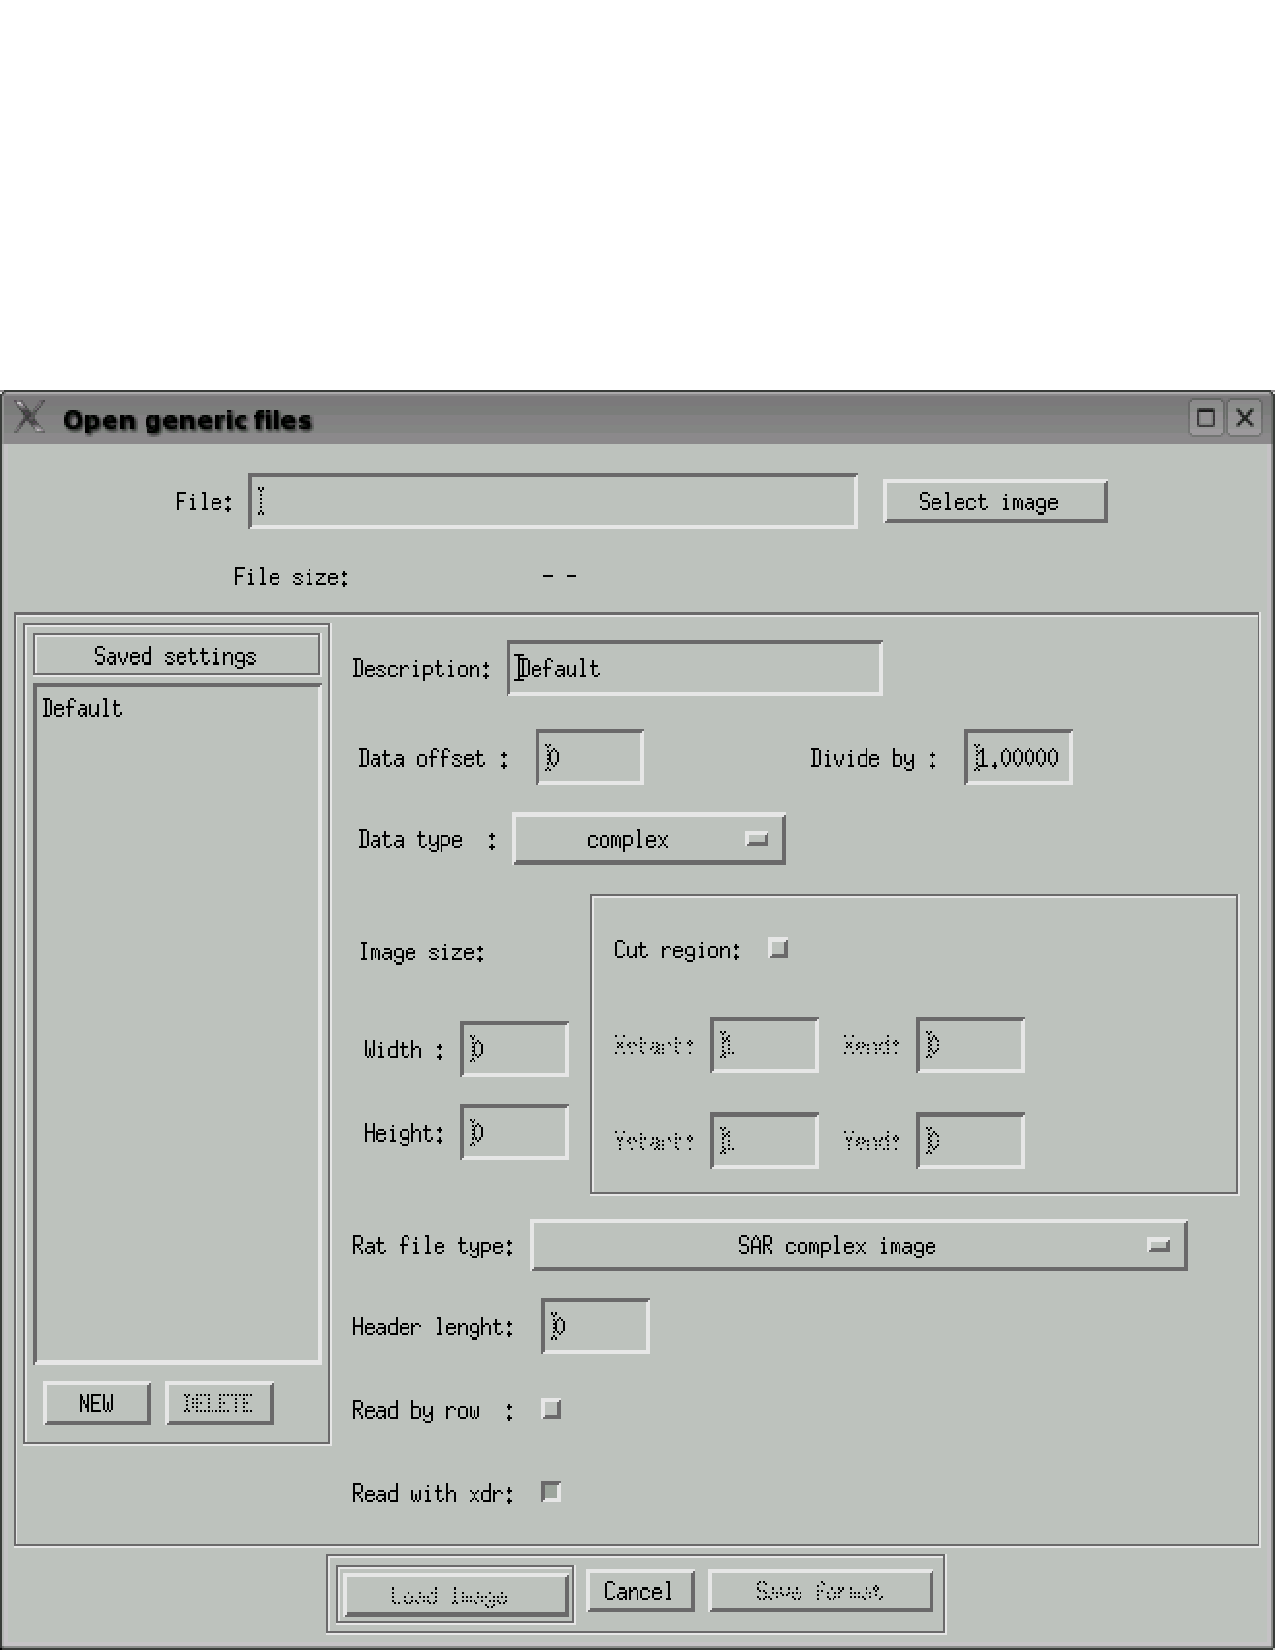
\includegraphics[scale=0.8]{images/pdf/import_gen.pdf}
%  \end{center}
%  
%  In this case, you have to specify:
%  
%  \begin{itemize}
%  
%  \item File: using the \verb*|Select image| button. At this point it will give you the size of the image.
%  
%  \item Description: you can choose a description name for you configuration if you have more than one file to open using \verb*|Open Generic Binary|. On the left side you can manage your different configuration.
%  
%  \item Data offset: you can add an global offset for all your data $new data = data + offset$.
%  
%  \item Divide by: you can divide the data by a global value.
%  
%  \item Data type: you can choose between the different kind of data existing.
%  
%  \item Image size: you have to specify the size of the image.
%  
%  \item Cut region: if you want to extract a sub image.
%  
%  \item Rat file type: define the type of file. Look at the chapter \ref{chapter:data_type} for more information.
%  
%  \item Header lenght: if your data have a header, you can specify here the lenght.
%  
%  \item Read by row: ???
%  
%  \item Read with \verb*|XDR|: allow to use the \verb*|/XDR| keyword when reading the data.
%  
%  \end{itemize}
%  
%  %=============================================================
%  \newpage 
%  %=============================================================
%  %=============================================================
%  %=============================================================
%  \section*{Open ENVI standart}
%  \addcontentsline{toc}{section}{Open ENVI standart}
%  
%  The standart ENVI file header (with \verb*|*.hdr| extension) has the following form:
%  
%  \begin{verbatim}
%  ENVI
%  description = {
%  unknown content.}
%  samples = 512
%  lines   = 512
%  bands   = 1
%  header offset = 0
%  file type = ENVI Standard
%  data type = 4
%  interleave = bip
%  sensor type = Unknown
%  byte order = 1
%  \end{verbatim}
%  
%  please, note that \verb|ENVI Standart| is specified to the \verb|file type| field.
%  
%  Up to now, only this header file is readable by RAT.
%  

\chapter{Single-channel SAR}


\section{Textures}

%---------------------------------------------------------------
\subsection{Variation coeffiecient}
%---------------------------------------------------------------

This function calculates the variation coefficient of an
amplitude or intensity SAR image. The variation coefficient
is defined as
%\be
\begin{equation}
  var = \frac{variance(x)}{mean(x)^2}
\end{equation}
%\ee
and is a measure of the amount of local gray-value variation.
In homogeoneous regions, its value is idependent of the 
local image amplitude; edges appear emphasized.

RAT allows to set the size in $x$ and $y$ of the box used
for estimation of variance and mean.

%---------------------------------------------------------------
\subsection{RFI filter}\label{sec:sarrfi}
%---------------------------------------------------------------

This routines (tries) to filter out so-called radio frequency interferences (RFI).
RFI come from received energy, which was not emitted by the SAR (mobile phones,
radio beacons, etc).

You have to set precisely some system parameters. RAT assumes the near range
to be on the left side of the displayed image! That's important. If the system
parameters are not precise, you can expect very stange filtering results. 

After starting the detection and waiting a bit, an image is shown, where potential RFI appear as
"white" spots. You can now use the sliders to adjust the notch filter. Ideally,
it should cancel out all the white spots (but not the rest). There are two filter parameters: The detection threshold sets the sensitivity
of detecting interferences. A value of 2.0 means that all RFI having an energy
of larger then 2.0 times the background are detected. The filter strength sets
the radius of the notch filter used for removing the detected RFI. A value of
3 means that a circle of radius 3 around the RFI peak is removed. You'll have to
press 'update window' if you want to see what'll happen when using the actual
filter parameters.

When you think your settings are fine, press "start filtering"....

\subsection{Co-occurence features}

\include{polar}
\chapter{Polarimetric Interferometry (PolInSAR)}

\section{Data Types}

RAT can handle polarimetric interferometric images. A POLInSAR image
pair is stored in a single file, in pixel interleave format.
The dimensions of data are: $N_x,N_y$ --- image dimensions; $N_{pol}$ --- number of
polarimetric channels (3 or 4), $N_{intrf}$ --- number of baselines (only 2
baselines are supported).

\begin{itemize}
  \item \emph{PolInSAR scattering vector}
    \[data = [ N_{intrf}; N_{pol}; N_x; N_y ]\]
  \item \emph{PolInSAR covariance matrix}
    \[data = [ N_{2pol}; N_{2pol}; N_x; N_y ]\qquad N_{2pol}=2*N_{pol}=N_{intrf}*N_{pol}\]
\end{itemize}


\section{Inspect}

%---------------------------------------------------------------
\subsection{Coherence Analysis}
%---------------------------------------------------------------
A variety of methods is used to visualize the POLInSAR coherence behavior in
dependence of averaging kind and quantity, computation methods, optimization
parameters, random coherence projections, etc. Compare \cite{cloude03:inversion,
colin03:cohopt, flynn02:cohshape, guillaso05:esprit, yamada01:esprit}.

\chapter{SAR Interferometry (InSAR)}
RAT can handle interferometric image pairs. An interferometric image
pair is stored in a single file, in pixel interleave format. 

%---------------------------------------------------------------
\section{Coregistration}
%---------------------------------------------------------------
Interferometric image pairs are usually not coregistered. Reasons
can be the baseline between the images, different range delays, shifted
image frames etc. As even a small misregistration drastically degrade the
coherence of an interferogram, before further processing a precise
coregistration has to be performed.

%---------------------------------------------------------------
\subsection{Global offset}\label{sec:insar_goff}
%---------------------------------------------------------------
This routine can shift the whole slave image by a constant offset.
The offset has to be an integer number, i.e. subpixel shifts
can not be performed with this routine. Enter the offset values in 
the upper box and press 'OK' to shift the slave image. 

If you don't know the image offset, you can use the "automatic offset
estimation" to estimate it. The default values in the boxes should be
o.k. for most cases. You have to change them only if you have images
with very large offsets. Shortly after "start estimation" has been pressed,
the estimated values appear in the upper box. Press "OK" to shift
the slave.

For offset estimation, the method of amplitude correlation is used. 
%---------------------------------------------------------------
\subsection{Subpixel offset}\label{sec:insar_soff}
%---------------------------------------------------------------
Very much the same as function \ref{sec:insar_goff}. A constant shift
of the entire slave image is performed, this time allowing floating point
values as offsets. For shifting, cubic interpolations are used.
It is not necessary to use this function when it is planned to use
"array of patches" or similar afterwards.

The estimation is based on oversampled amplitude correlation is used.
It is not possible to estimate very large offsets. In this case use
function \ref{sec:insar_goff} before.
%---------------------------------------------------------------
\subsection{Array of patches}\label{sec:insar_soff}
%---------------------------------------------------------------
This function estimates image offsets on a grid of small patches
distributed over the image. Then, a 2D-warping function is applied on
the slave image for coregistration. This function is useful if the
offsets are not constant over the image, which is often the case
in airborne repeat-pass images or spaceborne images with strong
topography.

In the first box, the number of patches and their size can be specified.
Don't select a too small size of the patches, since this will make the
results unreliable. Press "OK" to start the estimation.

After a while, a second box will appear showinh the vector field of
offsets. With the 2 edit buttons you can eliminate by hand obviously
wrong estimates. When everything looks good, press "Start coregistration"
to warp the slave image (time consuming!). Oversampling factors of 2 or 4
can help to better preserve image quality.

For offset estimation, oversampled amplitude correlation is used. For
warping, cubic convolution, is desired combined with FFT based 
oversampling, is used.

%---------------------------------------------------------------
%---------------------------------------------------------------
\section{Phase noise filter}
%---------------------------------------------------------------
%---------------------------------------------------------------
Phase noise filtering is used to enhance the quality of the interferometric
phase. It is usually employed prior to phase unwrapping, but can also be
useful for other purposes.
%---------------------------------------------------------------
\subsection{Boxcar}
%---------------------------------------------------------------
Boxcar filtering is a very simple filter: It is just a 
local averaging over the give rectangular box. Becuase of phase
wrapping effects, averaging is performed in the complex domain,
even if only a floating point phase is provided.
%---------------------------------------------------------------
\subsection{Goldstein}
%---------------------------------------------------------------
The Goldstein filter is a spectral filter which enhances
dominant fringe components in a local box. This is achieved by
multiplying the fringe spectra with its own amplitude power a
certain filter parameter (spectral exponent). Goldstein filtering
is very powerful in relatively high coherent regions, but might 
fail in low coherent areas.

In RAT, the window size is fixed to 64x64 pixels with an overlap
of 32 pixels.

%---------------------------------------------------------------
\subsection{GLSME}
%---------------------------------------------------------------
Another InSAR specific fringe filter. GLSME filtering minimises
globally the phase noise fluctuations by a least-squares approach.
GLSME seems to be very powerful especially for very low
coherent regions surrounded by high coherent areas.


%---------------------------------------------------------------
%---------------------------------------------------------------
\section{Coherence}
%---------------------------------------------------------------
%---------------------------------------------------------------
\subsection{Boxcar}
\subsection{Gauss}
\section{Remove flat-earth}
\subsection{linear}
\subsection{from file}
\section{Shaded relief}
\section{Transform}
\subsection{pair to interferogram}
\subsection{extract amplitude}
\subsection{extract phase}

\chapter{SAR Multichannel Subapertrues}

\section{Data Types}
The dimensions of data are: $N_x,N_y$ --- image dimensions; $N_{ap}$ --- number
of subapertures; $N_p$ --- number of vector elements in InSAR-, POLSAR-, POLInSAR- vectors.
\begin{itemize}
  \item \emph{Subapertures} Single channel subapertures
    \[data = [ N_{ap}; N_x; N_y ]\]
  \item \emph{Multi-channel Subapertures} Multichannel subapertures (e.g. for interferometry)
    \[data = [ N_{p}; N_{ap}; N_x; N_y ] \qquad N_p=N_{intrf}=2\mbox{ for interferometry}\]
  \item \emph{Polarimetric Subapertures} Multichannel subapertures for polarimetry
    \[data = [ N_{p}; N_x; N_y ] \qquad N_p=N_{pol}=\{3;4\}\]
  \item \emph{POLInSAR Subapertures} Multichannel subapertures for POLInSAR
    \[data = [ N_{p}; N_x; N_y ] \qquad N_p=N_{polin}=N_{pol}*N_{intrf}=\{6;8\}\]
    POLIn-channel order = $[ pol_0intrf_0;\ pol_1intrf_0;\ pol_2intrf_0;\ pol_0intrf_1;\ pol_1intrf_1;\ pol_2intrf_1]$
  \item \emph{Covariance matrices for every Subaperture}
    \[data = [ N_{p^2}; N_{ap}; N_x; N_y ] \qquad N_{p^2}=N_p^2=\{N_{pol}^2; N_{polin}^2\}\]
  \item \emph{Subapertures covariance matrix}
    \[data = [ N_{apcov}; N_{apcov}; N_x; N_y ] \qquad N_{apcov}=N_{p}*N_{ap}\]
  \item \emph{Subapertures stationarity [log(L)]} from \cite{ferro-famil03:subap}
    \[data = [ N_x; N_y ]\]
\end{itemize}

\section{Nonstationarity}

Evaluates the stationarity over azimuth subapertures. The result is
\emph{Subapertures stationarity [log(L)]}.\\
The nonstationary subapertures can be removed to generate a more stationary SAR image.
Compare \cite{ferro-famil03:subap}.

\chapter{Development Guide}

This section is meant as a reference for the developers of RAT, as well as for
those of you, who would like to understand better RAT was programmed.


\section{Import Template}

\section{Data Parameter Handling}
This section answers the questions:
\begin{itemize}
  \item How can I get access to parameters, resp. read/write them?
  \item How do I include new parameters.
  \item Where should I get the real parameters from?
\end{itemize}

\begin{enumerate}
  \item Define the parameter in the parameter structure \textbf{parstruct} in
    \textbf{definitions.pro}. The name of the entry is also the name of the
    parameter, followed by an NIL--Pointer type. Don't forget to add some
    comments about your parameter. Also think of a good name!
  \item For changing a parameter use the function \textbf{set\_par()}. You have to
    provide the name as a string and the value(can also be an array). As a
    result you get a status flag, which you should check. If you get 0, then
    everything is ok.
  \item For getting a parameter use the function \textbf{get\_par()}. See details above.
\end{enumerate}


\section{Speckle Filter Wizard}
This section answers the questions:
\begin{itemize}
  \item How do I include my newly written speckle filter into the Wizard.
  \item I have changed some parameters in my speckle filter. What do I have to
    modify in the Wizard?
\end{itemize}
Following modifications need to be considered:
\begin{enumerate}
  \item Put the name of the filter into the string--array
    \textbf{filter\_type}. Remember the position of your filter (index in the array).
  \item In dependence of the data type (POLINSAR, POLSAR, others) you should
    either \emph{offer} or \emph{not offer} this speckle filter to use. Set the right
    flag in the byte--array \textbf{offer}.
  \item Write generic fields for input in the widget at the right position.
  \item Call you speckle filter with the right parameters. Compere the fields
    you defined for the widget.
\end{enumerate}

\paragraph{Example}

\begin{enumerate}
  \item
\begin{verbatim}
  filter_type = [...,'MY-FILTER',...]  ; at position Z
\end{verbatim}
  \item
\begin{verbatim}
   POLINSAR --> offer = [...,1,...]  ; at position Z
   POLSAR   --> offer = [...,0,...]  ; at position Z
   OTHERS   --> offer = [...,0,...]  ; at position Z
\end{verbatim}
   with it this filter is allowed only for POLINSAR data
  \item 
\begin{verbatim}
Z: begin                ; MY-FILTER
   field[0,i]=CW_FIELD(filter_grp[i],VALUE=50,/integer,TITLE='Parameter1 : ',XSIZE=3)
   field[1,i]=CW_FIELD(filter_grp[i],VALUE=25,/integer,TITLE='Parameter2 : ',XSIZE=3)
\end{verbatim}
   \item
\begin{verbatim}
;; MY-FILTER
   Z: my-filter,/called,par1=*field_value[0],par2=*field_value[1]
\end{verbatim}
   \end{enumerate}
And that's it!


%\bibliographystyle{}
\bibliography{rat_references}
\bibliographystyle{unsrt}

\end{document}
